\section{Prepare for analysis}

\subsection{Correlation between features}

Understanding how features interact within the dataset is a key step before building predictive models. One effective way to explore these interactions is through correlation analysis. This technique reveals the strength and direction of linear relationships between variables, helping us detect redundant features, highlight those most relevant to the target variable, and optimize the feature set for better model efficiency and accuracy. By refining the input space early on, we set a strong foundation for the performance of our machine learning models.

One important aspect of correlation analysis is examining how strongly each feature relates to the target variable, in this case, Diabetes\_binary. Identifying variables that show a higher correlation with the target can guide us in selecting the most predictive features for our model. On the other hand, features that exhibit very weak relationships with the target may contribute little to the predictive power and can be excluded to simplify the model. Additionally, correlation analysis helps reveal whether certain features are highly related to each other. When two features show a strong correlation such as above 0.5 it may indicate redundancy. Retaining both could introduce multicollinearity, which not only complicates model interpretation but can also impair the algorithm’s performance. In such cases, it's often beneficial to remove one of the correlated features to streamline the dataset and enhance model robustness.

To calculate the correlation between features, we used the \texttt{corr()} function from the \texttt{pandas} library.  
We visualized the results using a Heatmap. A heatmap is a graphical representation that uses color gradients to indicate the strength of relationships in a two-dimensional matrix. This is especially useful for identifying patterns and connections between features.

The implementation can be seen in the code below, and the visual results are presented in Figure \ref{fig:correlation-matrix}:

\lstinputlisting[language=python]{../code/correlation.py}

\begin{figure}[H]
    \centering
oo    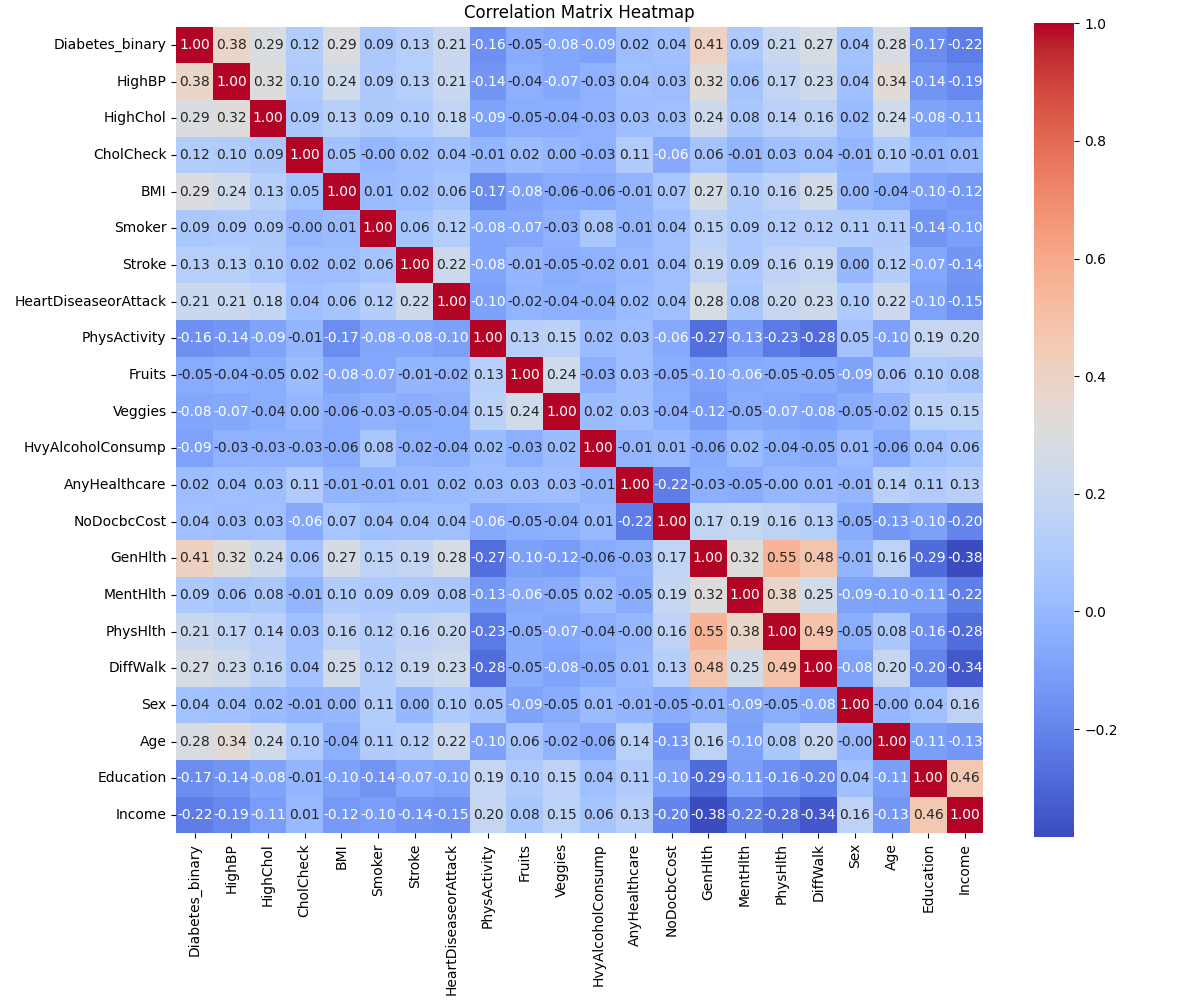
\includegraphics[width=0.7\textwidth]{images/diabetes_correlation_matrix.png}
    \caption{Correlation matrix between features.}
    \label{fig:correlation-matrix}
\end{figure}

From the heatmap visualization, we observe that some features are more strongly correlated with each other. We then filtered the feature pairs that have an absolute correlation higher than 0.45. The implementation of this filtering process in Python is shown below:

\lstinputlisting[language=python]{../code/correlation_filter.py}

The results are displayed in Table \ref{table:correlation-filtered}:

\begin{table}[ht]
\centering
\begin{tabular}{ |l|l|r| }
\hline
% \rowcolor{gray!30}
\textbf{Feature 1} & \textbf{Feature 2} & \textbf{Correlation} \\
\hline
GenHlth    & PhysHlth   & 0.552757 \\
PhysHlth   & DiffWalk   & 0.487976 \\
GenHlth    & DiffWalk   & 0.476639 \\
Education  & Income     & 0.460565 \\
\hline
\end{tabular}
\caption{Feature pairs with correlation $c > |0.45|$}
\label{table:correlation-filtered}
\end{table}
% \subsection{hej}
% To address weak correlation with the target variable, we will remove features exhibiting an absolute Pearson correlation coefficient of less than 0.1 with the 'Diabetes_binary' column. This step aims to eliminate features with a minimal linear relationship to the outcome we are trying to predict, potentially reducing noise and simplifying the model.

% Subsequently, to mitigate the issue of multicollinearity among the remaining features, we will identify pairs of features with a high absolute Pearson correlation coefficient (greater than 0.45). For each such pair, one of the features will be removed. The decision on which feature to remove will be based on its correlation with the target variable; the feature with the weaker absolute correlation to 'Diabetes_binary' will be prioritized for removal. This strategy aims to reduce redundancy in the feature set, which can lead to instability and interpretability issues in some models, without significantly sacrificing predictive power related to the target.
